\documentclass[
    book,tate,
    line_length=30zw,
    jafontsize=12pt,
    paper=b5j,
    landscape,
    ]{jlreq}
%図挿入用
\usepackage[dvipdfmx]{graphicx}
%ルビ用
\usepackage{pxrubrica}
%下の2行は目次のリンク用
\usepackage[dvipdfmx]{hyperref} 
\usepackage{pxjahyper}
%これはページ番号なくすため
\pagestyle{empty}
%余白設定用
%\usepackage{geometry}
%\renewcommand{\contentsname}{%
%\makebox[\linewidth]{\hfill 目\hspace{2zw}次\hfill}
%}
\title{\ruby{女教師}{おんな|きょう|し}と\ruby{淫鬼}{いん|き}【完全版】}
\author{\ruby{北都凛}{ほく|と|りん}}
\date{２０２６年４月１７日}

\begin{document}
\begin{center}
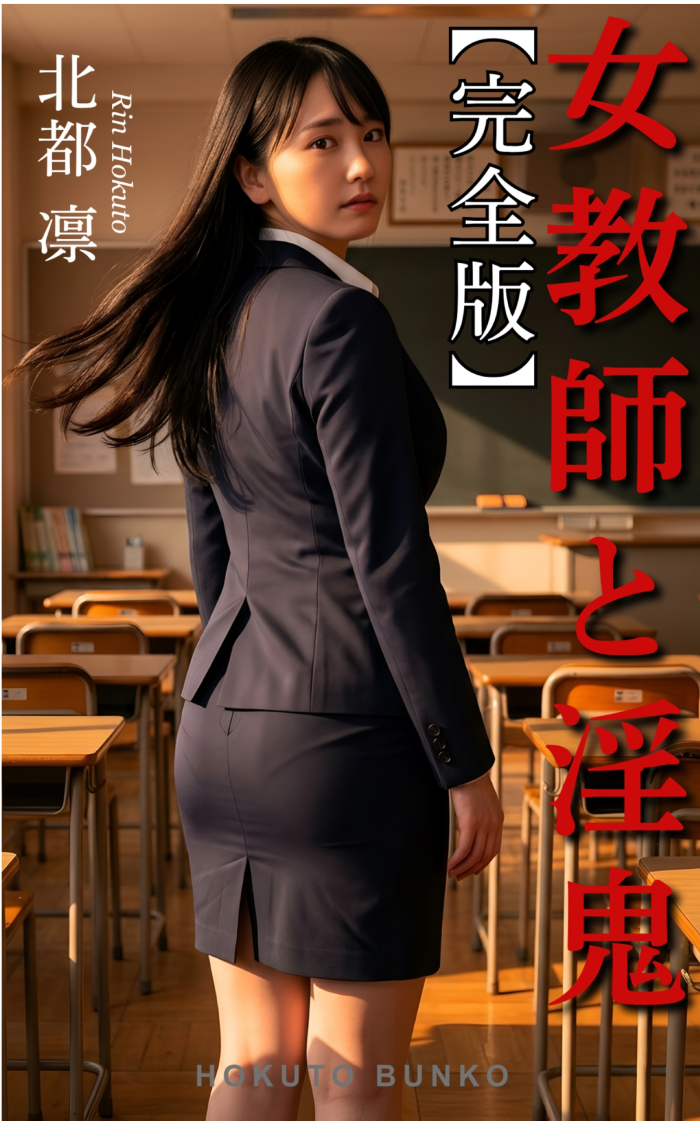
\includegraphics[angle=90,scale=0.45]{Onnakyoshi_Title.png}
\end{center}

\maketitle

\begin{center}
    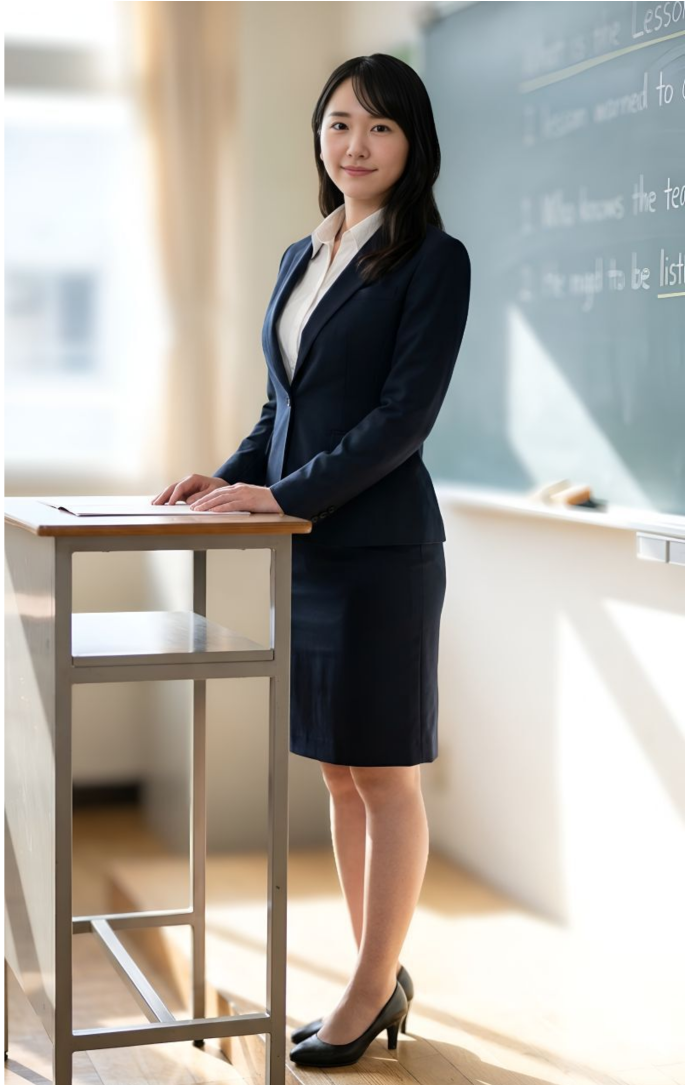
\includegraphics[angle=90,scale=0.45]{P00.png}
\end{center}

% 目次の出力
\tableofcontents

\chapter{プロローグ}

火曜日の朝------

人波に押されて乗りこんだ列車は、いつもの不快な熱気が充満していた。

他人同士が無言で体を密着させながらも、決して視線を合わせない。あらためて
見まわすと、なんとも異様な空間に思えてくる。

車内はスマートフォンのゲームに熱中する中年サラリーマンや吊革につかまって
目を閉じているＯＬ、それに窓の外をぼんやり眺めている制服姿の学生たちで
\ruby{鮨詰}{すし|づ}め状態だ。

レールの継ぎ目を通過する振動が、一定のリズムとなって眠気を誘う。

午前七時発の急行列車だ。あれほど苦手だった朝のラッシュも、いつの間にか
日常の光景となっているから不思議なものだ。

(もう五年も経つのね……)

人いきれでむっとする車両に揺られながら、\ruby{麻倉沙織}{あさ|くら|さ|おり}は
\ruby{感慨}{かん|がい}に\ruby{耽}{ふけ}っていた。

すでに三年生は卒業しており、在校生も終業式を一週間後に控えている。
教え子たちがそれぞれの思いを胸に新たな一歩を踏み出すこの季節、沙織は
まだ自分の将来を決めかねていた。

いったい、どれだけのことを伝えられたのだろうか。

受験のための英語を教えるだけではなく、ときには恋愛や進路の相談にも
乗ってきた。思春期の悩める若者たちと真正面から向き合い、無我夢中で
駆け抜けてきた五年間だった。

教え子たちの顔を一人ひとり思い浮かべるとき、教師という聖職に
\ruby{就}{つ}いた喜びを実感する。 まだ情熱が燃えつきたわけではない。
やはり今すぐに教職から離れるのは淋しいと感じていた。

(そろそろ、答えを出さないと……)

思わず息を小さく吐き出す。

その直後、列車がトンネルに入り、窓ガラスに自分の姿が映った。
\ruby{憂}{うれ}いをたたえたアーモンド形の瞳が\ruby{微}{かす}かに
揺れている。背中に垂れた黒髪は\ruby{艶}{つや}やかで、照明の光をキラキラと
反射していた。

ふと視線を感じて横を向く。すると、すぐ隣に立っている中年男が、じっとりと
湿った目で見つめていた。

(やだ……なに？)

\ruby{粘}{ねば}つくような視線が、胸もとを\ruby{無遠慮}{ぶ|えん|りょ}に這いまわる。

反射的に身をよじれば、濃紺のジャケットに包まれた大きな乳房がタプンッと揺れた。
コートの前をかき合わせると、咳払いをしてキッとにらみつける。 とたんに中年男は
ばつが悪そうに背中を向けた。

(まったく……)

この手のことにはなれているが、黙っている性格ではない。

モデル顔負けのプロポーションに女優を思わせる\ruby{華}{はな}やかな容姿は、
いつでも男の関心を惹きつけてしまう。

大学時代はミスキャンパスに四年連続で選ばれた\ruby{美貌}{び|ぼう}だ。
年月を\ruby{経}{へ}て二十七歳になり、美しさは\ruby{陰}{かげ}るどころか
ますます磨きがかかっていた。しかし、学園で教え子たちにちやほやされるのは
うれしいが、電車内で見知らぬ男に注目されるのは不快なだけだ。

(でも、教師を\ruby{辞}{や}めたら、こういうこともなくなるのね……)

それは喜ばしいことかもしれない。

だが、沙織の心は揺れていた。女の幸せを取るのか、教育者としてさらなる高みを
目指すのか。毎日そればかり考えていた。

大学時代の友人たちは、すでに何人か結婚している。輝く瞳で結婚生活を語る
彼女たちを見ていると、素直にうらやましく感じた。

(わたしも……)

教師を辞めて家庭に入ることを想像してみる。

\ruby{憧}{あこが}れはあるが、自分が主婦になった姿は今ひとつピンと来ない。
女の幸せをつかみたい気持ちはある。だが、教職に未練がないと言えば嘘になる。
やはり、結婚はもう少し先になるかもしれない。いずれにせよ、今すぐに答えを
出せることではなかった。

気を取り直そうと、満員の車内に視線をめぐらせる。

(あっ、白石さんだわ)

三人ほど乗客を挟んだ向こうに、見覚えのある小柄な女性が立っていた。

\ruby{襟}{えり}に白い三本のラインが入った伝統的な濃紺の制服は、
\ruby{星嶺学園}{せい|れい|がく|えん}のものに間違いない。ピンク色の
リボンで束ねられた黒髪のポニーテールが、斜めうしろの位置からはっきり
確認できた。

今どきめずらしい清楚な雰囲気の女子生徒は、二年生の
\ruby{白石結花}{しら|いし|ゆ|か}だ。

アイドルのような愛くるしい顔立ちをしており、男子生徒たちから絶大な
人気を誇っている。控えめでおとなしい性格のため\ruby{妬}{ねた}まれる
こともなく、同性の友人も多いようだ。

朝の電車でいっしょになって何度か言葉を交わすうちに、少しずつ結花の
純粋さに引きこまれた。 彼女と話すと心が洗われる気がする。結花も
\ruby{慕}{した}ってくれており、いつしか歳の離れた姉妹のような感情が
芽生えていた。

(なにかあったのかしら……)

幼さの残る横顔が、ふさぎこんで見えるのは気のせいだろうか。

結花はドアの横の\ruby{手摺}{て|す}りにつかまり、うつむき加減に立って
いる。窓から射しこむ日の光が、黒目がちの潤んだ瞳を照らしていた。


\section*{\tatechuyoko{1}}

\rightline{(了)}
\end{document}
